



\section{Preliminaries}


Given a pretrained language model $G$ and the original training data of a task $\mathcal{D}_{\text{SFT}} = \{(x_1, y_1), (x_2, y_2), \cdots (x_N, y_N)\}$, where $x$ is typically a description of a problem and $y$ is the solution, such as chain-of-thought rationale or generated code. 
The de facto approach for such tasks 
 with causal language models is supervised fine-tuning (SFT) with the negative log-likelihood objective on the training data:
\begin{equation}
\label{eq:sft}\mathcal{L}_{\text{SFT}}(G) = -\E_{(x,y)\sim \mathcal{D}_{\text{SFT}}} \sum\limits_{t=1}^{T} \log G (y_t \mid y_{<t}, x)
\end{equation}
where $G$ is also referred to as \textit{generator} in reasoning tasks. % With high quality generations at inference one could further improve the model.
LLMs can be used to generate high quality chain-of-thought rationales or solutions for a range of tasks. 
This observation has motivated using correct generations from the model itself to bootstrap problem-solving and reasoning abilities~\citep{DBLP:conf/nips/ZelikmanWMG22, singh2023human, yuan2023scaling}.

\begin{table*}[t!]
% \vspace{-1.5em}
\caption{Comparison of  self-improvement and verification methods, showing the data used to train the generator and verifier (if applicable), and whether or not the method is iterative.}
\vspace*{-1em}
\label{tab:bootstrap_methods}
\begin{center}
% \begin{footnotesize}
\begin{sc}
\footnotesize
\begin{tabular}{@{}lllr}
\toprule
Method & Generator Data & Verifier Data & Iterative \\
\midrule
SFT & $\mathcal{D}_{\text{SFT}}$  & \xmark & \xmark \\
Verification & $\mathcal{D}_{\text{SFT}}$  & $\mathcal{D}_{\text{SFT}}$ $\cup$ Generated & \xmark \\
STaR & $\text{Correct Generated}_{t-1}$ & \xmark & \cmark \\
RFT~(\stardag[1 iter]) &  $\mathcal{D}_{\text{SFT}}$ $\cup$ Correct Generated & \xmark & \xmark \\
\stardag & $\mathcal{D}_{\text{SFT}}$ $\cup$ $\text{Correct Generated}_{<t}$ & \xmark & \cmark \\\midrule
\vstar{} [1 Iter] & $\mathcal{D}_{\text{SFT}}$ $\cup$ Correct Generated & $\mathcal{D}_{\text{SFT}}$ $\cup$  Generated & \xmark \\
\textbf{\vstar{}} & $\boldsymbol{\mathcal{D}}_{\textbf{SFT}}$ $\boldsymbol{\cup}$ $\textbf{Correct Generated}_{\boldsymbol{<t}}$ & $\boldsymbol{\mathcal{D}}_{\textbf{SFT}}$ $\boldsymbol{\cup}$ $\textbf{Generated}_{\boldsymbol{<t}}$ & \textbf{\cmark} \\
\bottomrule
\end{tabular}
\end{sc}
% \end{footnotesize}
\end{center}
\vskip -0.1in
\end{table*}


\subsection{Self-improvement approaches}
\label{sec:si_approach}

\textbf{Self-Taught Reasoner}~\citep[STaR;][]{DBLP:conf/nips/ZelikmanWMG22} corresponds to an iterative approach where a language model improves itself using correctness feedback.
In each iteration, \revision{one solution $\hat{y}$ is generated using greedy decoding from the generator $G$ }for each problem $x$ in training dataset $\mathcal{D}$.
Having access to test cases or ground truth answers, generated solutions can be checked for their binary correctness label $z$ \revision{by
$z = \text{is\_correct}(x,\hat{y}), \qquad z \in \{0, 1\}.$}
A completion $\hat{y}$ is labeled correct if it has the same final answer as the ground truth answer for math problems, or if it passes all the test cases for code generation problems.
Only correct solutions ($z = 1$) are included in the dataset at iteration $j$ where $\mathcal{D}_j = \{(x_1, \hat{y}_1), (x_2, \hat{y}_2), \cdots (x_N, \hat{y}_N)\}$.
Then, the generator is fine-tuned on this new dataset using (\autoref{eq:sft}) where $\mathcal{D}_{\text{SFT}} = \mathcal{D}_j$. This fine-tuned generator is used in subsequent iterations. 


\textbf{Rejection Sampling Fine-tuning}~\citep[RFT;][]{yuan2023scaling} first fine-tunes a pretrained LM on the training dataset $\mathcal{D}_{\text{SFT}}$ to obtain $G$. For each problem $x_i$, \revision{$k$ solutions are sampled $\{\hat{y}_{i,j} \sim G (y|x_i) \}_{j=1}^k$} and similar to STaR, \revision{only correct generated solutions ($z=1$) are kept}. In RFT, the original dataset is then augmented with the correct completions to $\mathcal{D}_j$, and $G$ is fine-tuned on the new $\mathcal{D}_j$ to obtain $G_{\text{RFT}}$. Unlike STaR, RFT is not an iterative approach.

\textbf{\stardag}. Each STaR iteration can be performed similarly to RFT, akin to ReST$^{EM}$~\citep{singh2023human}. Since there could be multiple correct solutions for a problem, one could sample $k$ solutions per problem at each STaR iteration, \revision{but this is not prescribed in the original STaR paper, which we will denote as \stardag for the rest of the paper.}

% . For the rest of the paper, we denote this variant of STaR as \stardag. 
% Performing only 1 iteration of \stardag~corresponds to RFT.



\subsection{Test-time verification}
\label{sec:orm}
\citet{DBLP:journals/corr/abs-2110-14168} trained verifiers, which they refer as outcome-supervised reward model (\textbf{ORM}), that assess the probability that a candidate solution is correct for a given problem.  At test time, 
the language model $G$ generates many candidate solutions and the one ranked highest by the verifier is selected, also known as \textbf{Best-of-k}. To train a verifier $V$, similar to RFT, $k$
 candidate solutions are sampled from a generator $G$ for each training problem and labeled for their correctness $z$ to make the verifier training data $\mathcal{D_\text{VER}} = \{(x_i, \hat{y}_{i,j}, z_{i,j})\}_{i=1}^{N}$, where $z_{i,j}$ is a binary label indicating whether $\hat{y}_{i,j}$ is a correct or incorrect solution. 
 
To train the verifier $V$, \citet{DBLP:journals/corr/abs-2110-14168} fine-tune a LLM on $\mathcal{D_\text{VER}}$ using a combination of language modeling (\autoref{eq:sft}) and binary classification. The model is trained to predict $\hat{y}_{i,j}$
 given $x_i$ and $z_{i,j}$ given $\{x_i;\hat{y}_{i,j}$\} with the language modeling and the classification objective, respectively. See \autoref{sec:related} for more details.


\subsection{Preference learning with DPO}
\label{sec:dpo_obj}
Fine-tuning pretrained LLMs with human feedback can result in large performance gains in downstream tasks \cite{DBLP:conf/nips/Ouyang0JAWMZASR22, bai2022constitutional}. The typical framework to do so is to collect paired human preferences for a set of input prompts $\mathcal{D}_{\text{pref}} = \{(x_i,y_i^{+}, y_i^{-})\}_{i=1}^{N}$, 
train a reward model using $\mathcal{D}_{\text{pref}}$, and fine-tune the LLM using this reward~\citep{DBLP:journals/corr/abs-2009-01325}.

More recently, \citet{rafailov2023direct} proposed Direct Preference Optimization (DPO), which does not use a separately trained reward model during fine-tuning. DPO requires supervised fine-tuning (SFT) a pretrained LLM on the downstream task to obtain $G_{\text{SFT}}$, which is also \revision{ used as a reference policy}. 
Given the preference dataset $\mathcal{D}_{\text{pref}}$ and $G_{\text{SFT}}$, DPO's objective increases the log likelihood, relative to the reference policy,  of preferred $y^+$ to dispreferred $y^-$ completions. We present the DPO loss later in \autoref{eq:dpo}, in the context of training verifiers.

% \begin{multline}
%     \mathcal{L}_{\text{DPO}}(V; G_{\text{SFT}}) = \\
%     - \E_{(x, y^+, y^-) \sim \mathcal{D}_{\text{pref}}} \left[ \log \sigma \left( \hat{g}(x,y^+) -  \hat{g}(x,y^-) \right) \right]
% \end{multline}
% Where $\hat{g}(x,y) = \beta \log \frac{V (y | x)}{G_{\text{SFT}}(y | x)}$, $\sigma$ is the logistic function, and $\beta$ is a hyper-parameter controlling the proximity to the reference policy $G_{\text{SFT}}$.





\section{\vstar{}: Verifiers for self-taught reasoners}

Existing self-improvement methods, such as RFT, STaR, and $\text{ReST}^{EM}$, throw away \revision{incorrect model-generated solutions}. However, incorrect solutions can also contain valuable information: a language model could learn from discrepancies between correct and incorrect solutions for a given problem, and identify error patterns in generations, enhancing its ability to provide more accurate solutions.  
In this work, we propose \textbf{\vstar{}} that utilizes both incorrect and correct generated solutions in an iterative process to train a better generator and verifier (see \autoref{alg:vstar} in appendix).   
\begin{figure*}[t]
\vspace*{-1.6em}
\centering
\begin{subfigure}[b]{0.5\textwidth}
  \centering
  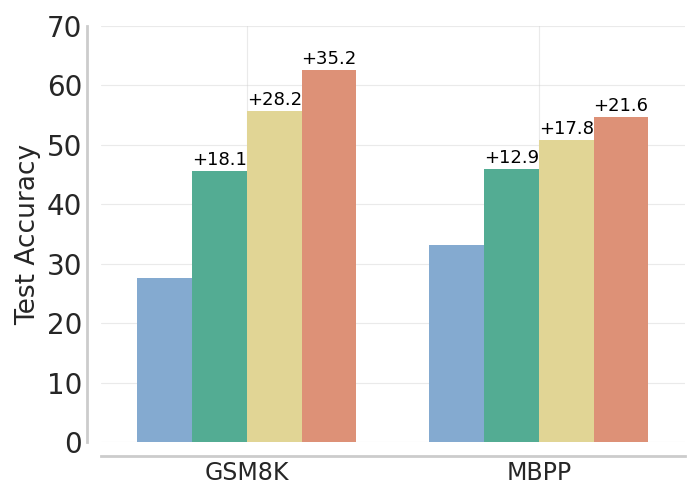
\includegraphics[scale=0.39]{icml2023/figs/benchmark_7B/bechmark_train_7B.png}
  % \caption{Tasks}
    \label{fig:main_tasks}
\end{subfigure}%
\begin{subfigure}[b]{0.5\textwidth}
  \centering
  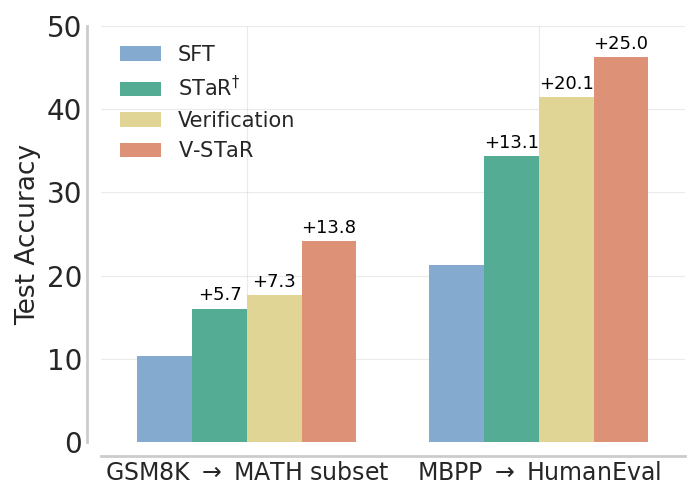
\includegraphics[scale=0.39]{icml2023/figs/benchmark_7B/bechmark_transfer_7B.png}
  % \caption{Transfer tasks}
    \label{fig:transfer_main}
\end{subfigure}%
\vspace*{-1em}
\caption{\textbf{Test accuracy of 7B \vstar{} compared to self-improvement and verification baselines.} 
We report Best-of-64 for verification-based methods and Pass$@1$ for others. All methods, except SFT, have access to the SFT baseline model and $K=48$ output generations per problem. \stardag{} and \vstar{} are run for 3 iterations, where each iteration uses $K/3 = 16$ samples. Verification corresponds to using a test-time verifier trained on K generated completions from the SFT generator. Numbers above each bar show the absolute improvement over SFT. \textbf{(Left)} Test accuracy on  tasks used for \vstar{} training. \textbf{(Right)} Transfer evaluation of GSM8K and MBPP trained models on MATH subset and HumanEval respectively.}
\label{fig:results}
\vspace{-0.1in}
\end{figure*}


\begin{itemize}[left=0pt,itemsep=2pt,topsep=2pt]
\item First, we fine-tune a pretrained LLM $G_{\text{base}}$ on the original training data $\mathcal{D_\text{SFT}}$ to obtain generator $G_{\text{SFT}}$.  


\item Next, we sample $k$ completions for each problem in the training data from the generator $\{\hat{y}_{i,j} \sim G (y|x_i) \}_{j=1}^k$, where $x \in \mathcal{D}_
{\text{query}}$ (see~\autoref{app:gsm_candidates} for an example). 

\item Generated solutions are labeled for their correctness $z$ using ground truth answers or test cases. We use only correct generated solutions ($z=1$) to augment the generator training data $\mathcal{D_\text{GEN}}$ as $(x_i, \hat{y}_{i,j})$.
Both correct and incorrect generated solutions are added to verifier data $\mathcal{D_\text{VER}}$ with their correctness label  as $(x_i, \hat{y}_{i,j}, z_{i,j})$, so the verifier can learn from generator's mistakes. 
% We chose to augment our datasets following~\citet{gulcehre2023reinforced}.

\item In the next iteration $t$, the generator $G^{t}$ is obtained by fine-tuning the pretrained model $G_{\text{base}}$ on the augmented $\mathcal{D_\text{GEN}}$. We can sample solutions again from this generator $G^{t}$. This process is repeated for up to $T$ iterations to augment $\mathcal{D_\text{GEN}}$ and $\mathcal{D_\text{VER}}$ iteratively. 

\item The final generator $G^T$ is obtained by using $\mathcal{D_\text{GEN}}$ to fine-tune a pretrained model $G_{\text{base}}$.
The verifier $V^T$ is obtained by using $\mathcal{D_\text{VER}}$ to further train a model $G_{\text{SFT}}$ which was fine-tuned on the original $\mathcal{D_\text{SFT}}$.

\end{itemize}

In our approach, the original training data is also included as correct solutions in both generator data and verifier data.
The difference between \vstar{} training and \citet{DBLP:journals/corr/abs-2110-14168} is that our verifier training data is collected iteratively, each iteration from a better generator, while ORM only collects data from a fixed generator that is only fine-tuned on the original SFT data. We compare to this ORM approach as a baseline, as discussed in \autoref{sec:baselines}.


% \vspace{-0.08in}
\subsection{Training verifiers with DPO}
\label{sec:dpo_verifier}

Following \citet{DBLP:journals/corr/abs-2110-14168},
current LLM verifiers are trained with a combination of language modeling and binary classification loss (\autoref{sec:orm}). These two objectives can be unified via offline preference learning methods, such as DPO~\citep{rafailov2023direct}, where the proximity to the reference policy is a proxy for the language modeling objective while the classification loss is a proxy for reward modelling. Empirically, we found DPO verifiers to be better than ORM-style verifiers~(\autoref{sec:dpo}), when using LoRA adapters~\citep{DBLP:conf/iclr/HuSWALWWC22}.

To use DPO for training verifiers, we construct a preference pair dataset using collected solutions in $\mathcal{D_\text{VER}}$. We treat correct solutions as preferred and incorrect solutions as not preferred completions given the problem.
Specifically, $\mathcal{D_\text{VER}} = \{(x_i,y_{i,1}^{+}, y_{i,1}^{-}), \cdots ,(x_i,y_{i,m}^{+}, y_{i,m}^{-})\}_{i=1}^{N}$, where $m$ is the number of preference pairs which are from the Cartesian product of correct and incorrect solutions.
% $$(y_{i}^{+}, y_{i}^{-}) \in \{\hat{y}_{i,j} \mid z_{i,j} = 1\} \times \{\hat{y}_{i,j} \mid z_{i,j} = 0\}.$$
We train our verifier $V$ using this constructed $\mathcal{D_\text{VER}}$ and the SFT policy $G_{\text{SFT}}$ using the DPO objective, $\mathcal{L}_{\text{DPO}}(V; G_{\text{SFT}})$: 
\begin{align}
    - \E_{(x, y^+, y^-) \sim \mathcal{D}_{\text{VER}}} \left[ \log \sigma \left( \hat{r}(x,y^+) -  \hat{r}(x,y^-) \right) \right], \quad \mathrm{with}\  \hat{r}(x,y) = \beta \log \frac{V (y | x)}{G_{\text{SFT}}(y | x)} \label{eq:dpo}
\end{align}
where $\sigma$ is the logistic function, and $\beta$ is a hyper-parameter controlling the proximity to the reference policy $G_{\text{SFT}}$.
The DPO objective steers the verifier towards increasing the likelihood of correct solutions $y^+$ and decreasing the likelihood of incorrect solutions $y^-$ for a problem $x$.
% Note that the DPO objective combines 
% for more details.
At inference, we use the likelihood of a generated solution given a problem under the trained DPO verifier~(i.e. $V(\hat{y} | x)$) as scores to rank candidate solutions. 




